\documentclass[12pt, a4paper]{report}
\linespread{1.3}
\setlength{\parindent}{1.25cm}

\usepackage[top=3cm,left=3cm,right=2cm,bottom=2cm]{geometry}
\usepackage{indentfirst}
\usepackage{amsmath, amsthm, amsfonts, amssymb}

\usepackage{graphicx}
\usepackage{color}
\usepackage{multicol}
\usepackage[normalem]{ulem}
\usepackage{wrapfig}
\usepackage{caption}
\usepackage{fancybox}
\usepackage[pdfstartview=FitH]{hyperref}
\usepackage{subfigure}

\usepackage[T1]{fontenc}		% Selecao de codigos de fonte.
\usepackage[utf8]{inputenc}
\usepackage[brazil]{babel}

\usepackage{array}
\usepackage{longtable}
\usepackage{pdfpages}

\usepackage{verbatim}
\usepackage{enumitem}          % criação de linhas

%Includes "References" in the table of contents
\usepackage[nottoc]{tocbibind}

\graphicspath{{Figuras/}} % caminho padrao imagens
% ------ Remove nome capitulo da tag chapter ---------
\makeatletter
\def\@makechapterhead#1{%
  \vspace*{0\p@}%
  {\parindent \z@ \raggedright \normalfont
    \interlinepenalty\@M
    \Huge\bfseries  \thechapter.\quad #1\par\nobreak
    \vskip 30\p@
  }}
\makeatother
\begin{document}

%---------- CAPA -------------

\begin{figure}[ht]
\centering

\includegraphics[scale=0.15]{UFBA.jpg}
\end{figure}

\begin{center}
\sc{\large{Universidade Federal da Bahia - UFBA}} \\
\sc{\large{Instituto de Matematica - IM}} \\
\sc{\large{Departamento de Ciência da Computação - DCC}} \\
\sc{\small{Bacharelado em Sistemas de Informação - BSI}} \\
\sc{\small{Trabalho de Conclusão de Curso}} \\

\vspace{4cm}

\sc{\Large{Desenvolvimento e Avaliação\\do SICAD - UFBA}}

\vspace{4.5cm}

\sc{\Large{Kênia Arruda Guimarães}}

\vspace{5.5cm}

\textbf{Salvador - Bahia} \\
Dezembro de 2019

\end{center}

%---------- FOLHA DE ROSTO -------------
\newpage
\begin{center}
\sc{\Large{Desenvolvimento e Avaliação\\do SICAD - UFBA}}

\vspace{4cm}

\large{Kênia Arruda Guimarães}
\end{center}

\vspace{4cm}

\begin{flushright}
\begin{minipage}{8.6cm}
Monografia apresentada como trabalho de conclusão de curso para o curso de Bacharelado em Sistemas de Informação do Departamento de Ciência da Computação na Universidade Federal da Bahia.

\vspace{0.5cm}
\textbf{Orientador}: Prof. Dr. Rodrigo Rocha Gomes e Souza.

\end{minipage}
\end{flushright}
 
\vspace{8cm}


\begin{center}
\textbf{Salvador - Bahia} \\
Dezembro de 2019
\end{center}

\presentationpage

%%%%%%%%%%%%%%%%%%%%%%
% Ficha Catalográfica
\newpage
\thispagestyle{empty}
\null\vfill
                  
\begin{center}
 Ficha catalográfica.
\begin{tabular}{|p{13.5cm}|}%{p{12cm}}
\hline
\begin{small}
\begin{verbatim}
Guimarães, Kênia Arruda
Desenvolvimento e Avaliação do SICAD-UFBA. / Kênia
Arruda Guimarães. - Salvador, 01, 2008.

182p.:il.
Orientador: Rodrigo Rocha Gomes e Souza.

Monagrafia (Graduaçao) -UNIVERSIDADE FEDERAL DA BAHIA,
INSTITUTO DE MATEMÁTICA, 06 de abril de 2017.

TOPICOS PARA FICHA CATALOGRAFICA.I. 
Souza, Rodrigo Rocha Gomes e. II. UNIVERSIDADE FEDERAL DA BAHIA. 
INSTITUTO DE MATEMÁTICA. III Título.
                                                  NUMERO CDD
\end{verbatim}
\end{small}
\\ \hline
\end{tabular}
\end{center}
\setcounter{page}{2} %truque para não numerar a página


%---------- BANCA EXAMINADORA -------------
\newpage
\begin{center}
\sc{\Large{Desenvolvimento e Avaliação\\do SICAD - UFBA}}

\vspace{2.2cm}

\large{Kênia Arruda Guimarães}
\end{center}

\vspace{2.2cm}

\begin{flushright}
\begin{minipage}{8.6cm} 
Monografia apresentada como trabalho de conclusão de curso para o curso de Bacharelado em Sistemas de Informação do Departamento de Ciência da Computação na Universidade Federal da Bahia.
\end{minipage}
\end{flushright}
 
\vspace{1cm}
\begin{center}
\Large \textbf{Banca Examinadora:}
\end{center}
\vspace{1.5cm}

\begin{flushright}
\begin{minipage}[l]{12cm}
\begin{center}
\uline{\hspace{10.5cm}} \\
Prof. Dr. Rodrigo Rocha Gomes e Souza (Orientador) \\ Universidade Federal da Bahia \\
\vspace{1cm}
\uline{\hspace{10.5cm}} \\

\vspace{1cm}
\uline{\hspace{10.5cm}} \\


\end{center}
\end{minipage}
\end{flushright}

%-----------Dedicatória----------------
\newpage
\vspace*{21cm}
\begin{flushright}
\textit{Dedico este trabalho à minha família}
\end{flushright}


%------------Agradecimentos------------
\newpage
\chapter*{Agradecimentos}
\thispagestyle{empty}
\par Aos meus pais que sempre estiveram ao meu lado me apoiando em cada decisão tomada. À minha noiva Juliana Alves Pereira que vem sendo meu maior suporte neste ciclo de aprendizado. À minha amiga Lina Mendes que me deu grande auxílio no design da aplicação. Aos meus amigos e em especial a Carlos Henrique e Ludmila Cruz que sempre tiveram muita paciência ao ouvir os desabafos quando ainda não tinha encontrado a solução para alguns dos obstáculos que encontrei durante a a execução deste projeto. E por fim, ao meu orientador Rodrigo Rocha Gomes e Souza pela excelente orientação, paciência e atenção prestados no desenvolvimento deste trabalho e a Universidade Federal da Bahia (UFBA) pelo espaço público de ensino que mesmo com todas as dificuldades encontradas forma profissionais excelentes que trarão conhecimento contribuindo para o desenvolvimento do nosso país.  

%------------Citação-------------------
\newpage
\vspace*{20cm}
\begin{flushright}
\begin{minipage}{7cm}
\begin{flushright}
\textit{
"Toda a ciência é nada mais do que um refinamento do pensamento cotidiano". \\
Albert Einstein}
\end{flushright}
\end{minipage}
\end{flushright}


%--------------Resumo-------------------
\newpage
\chapter*{Resumo}
\thispagestyle{empty}


%-------------Abstract------------------
\newpage
\chapter*{Abstract}
\thispagestyle{empty}

%-------------Índice--------------------
\newpage
\tableofcontents
\thispagestyle{empty}

% ----------- Lista de figuras ----------

\pdfbookmark[0]{\listfigurename}{lof}
\listoffigures
\cleardoublepage

%--------- Lista de tabelas ---------

\pdfbookmark[0]{\listtablename}{lot}
\listoftables
\cleardoublepage

%-------------Capítulo 1-----------------
\chapter{Introdução}

%-------------Capítulo 2-----------------
\chapter {Trabalhos Relacionados}

%-------------Capítulo 3-----------------
\chapter{Solução Proposta: SICAD}
\par Como solução para a problemática apresentada neste trabalho está sendo proposto o Sistema Colaborativo de Avaliação Docente, SICAD, como ferramenta auxiliar para os discentes da Universidade Federal da Bahia utilizarem, a fim de disponibilizar seus feedbacks e avaliações sobre as disciplinas cursadas pelos mesmos. 
\par O processo de concepção do SICAD foi realizado inicialmente como uma junção do trabalho já realizado pelo Sistema de Avaliação Docente, o SIAV, da UFBA  mais a funcionalidade dos comentários. A partir deste escopo foram traçados os requisitos da solução que serão descritos abaixo.

\section{ Modelo Conceitual}
\section{ Autenticação}
\par Inicialmente foi pensado em um login básico para autenticação no sistema. Contudo, analisando o contexto, a cenário abrangeria qualquer usuário logado na internet que possuísse o caminho do sistema, não sendo interessante pois os mesmos teriam acesso a resultados que possuem informações sensíveis.
\par Para delimitar o acesso ao SICAD, foi utilizado o módulo de autenticação disponibilizado pela UFBA no caminho https://www.autenticacao.ufba.br. Sua utilização segue o seguinte processo: a aplicação no momento do login faz uma requisição à autenticação e a mesma retorna o username caso o usuário possua cadastro na universidade. Segue abaixo o fluxograma do processo.
\begin{figure}[!ht]
\centering
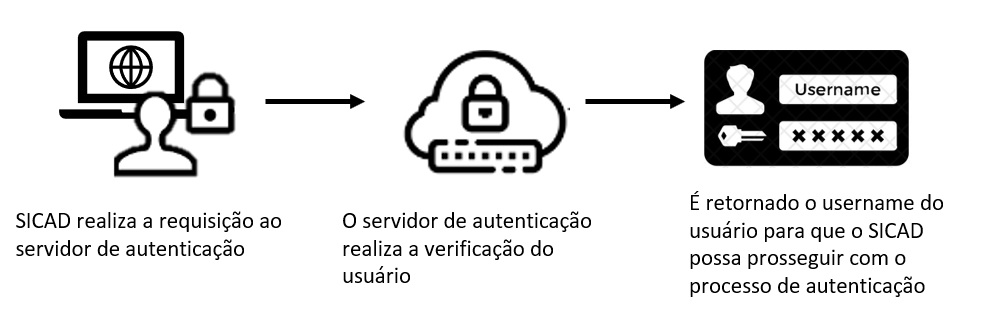
\includegraphics[scale=0.50]{processo_autenticacao.jpg}
\caption{Fluxograma da Requisição de Autenticação}
\label{fig:processo_autenticacao}
\end{figure}

\par Dessa forma o acesso fica restrito a quem possuí cadastro na universidade não expondo assim informações indevidas a usuário que não são elegíveis para utilizar o SICAD.

\subsection{Usuário e Segurança}
\par No processo de desenvolvimento  da autenticação ficou claro a necessidade da implementação de uma camada de segurança, visto que a resposta à requisição feita juntamente a UFBA retorna o username do usuário sem nenhum tipo proteção.
\par A segurança da informação é essencial no sentido de preservar o valor dessa informação que é chave para a maioria das funcionalidades do SICAD. Focanalizando neste ponto foram implementadas rotinas para prover segurança nos processos executados pelo sistema que será descrito abaixo:

\begin{itemize}
\item o usuário tenta logar no sistema, consequentemente disparando uma requisição para a autenticação da UFBA;
\item A ufba executa todos as rotinas de validação.
Caso postivo, retorna o username do usuario sem criptografia;
\item O SICAD antes de persistir a informação  no banco de dados, utiliza da tencologia de criptografia Hash SHA256, que será abordada no topico 3,6. para encriptografar o username será chave para utilização do sistema..
\end{itemize}
\par Por conseguinte, com o usuário criptografado a integridade da informação estará mantida seno assim confiavel que o usuario a utilize sem preocupações

\section{ Perfis}
\par
\section{ Moderação}
\section{ Anonimato}
\section{ Segurança}
\section{ Principais Funcionalidades}

%-------------Capítulo 4-----------------
\chapter{Considerações Finais}

%-------------Bibliografia------------------

\renewcommand\bibname{Referências}
\bibliographystyle{unsrt}
\bibliography{referencias}
\nocite{*}

%-------------Apêndice------------------
\appendix

\end{document}
